\chapter{Evaluation}\label{chap:evaluation}

Clearly not every project has empirical components (in particular in mathematics or theoretical topics) -- though many do. So in case you were coding anything and conducted an empirical evaluation, this is where you should report the results.

As always, make adequate use of sections/subsections to structure this chapter. 
These are some suggestions on what you may report on:
\begin{itemize}
  \item Benchmark Selection: Which data set did you choose to evaluate your approach on? Why did you make that specific selection? Would there have been alternatives?
  \item Hardware setup: What hardware was used (processor, RAM, etc.), and which operating systems and software were used?
  \item Results: Report the plain data (plots, tables, etc.)\ and their \emph{interpretation}, i.e., did the approach work well or not? Do we know on which subset it worked well (or badly) and why was it like this? Do the results raise further questions and thus directions for future research/investigations?
\end{itemize}

When reporting your results using graphs and plots, make sure to provide all information necessary to interpret the data, e.g., axis and graph labeling (cf.~Figure~\ref{fig:xkcd}).


  \begin{figure}[bh!]
  \floatbox[{\capbeside\thisfloatsetup{capbesideposition={left,top},capbesidewidth=.5\textwidth}}]{figure}[\FBwidth]
  {\caption{A graph illustrating the importance of axis and graph labeling. (Graphic taken from \url{https://xkcd.com/252/}.)\label{fig:xkcd}}}
  {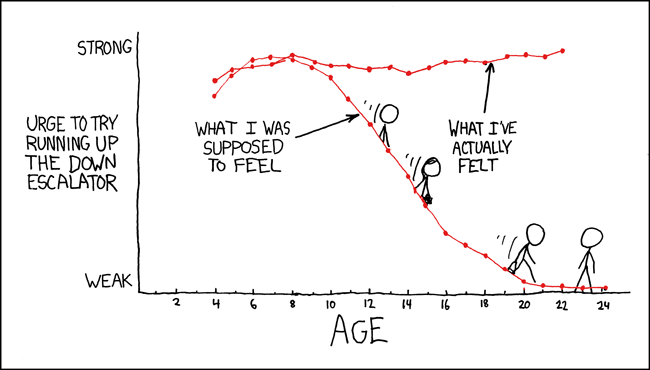
\includegraphics[width=.5\textwidth]{figures/escalators.png}}
  \end{figure}


% \begin{figure}%
%   \fbox{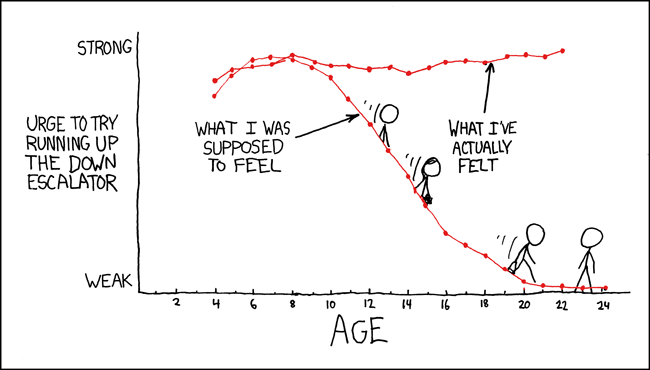
\includegraphics[width=.2\textwidth]{figures/escalators.png}}
%   \caption{An example graph illustrating the importance of captions and axis labeling. (Graphic taken from \url{https://xkcd.com/252/}.)\label{fig:xkcd}}
% \end{figure}%
